\documentclass{article}
\usepackage[utf8]{inputenc}
\usepackage{tikz}
\usepackage{natbib}
\usepackage{graphicx}
\usepackage{amsmath}
\usepackage{verbatim}
\usepackage{hyperref}
\hypersetup{
    colorlinks=true,
    linkcolor=blue,
    filecolor=magenta,      
    urlcolor=blue,
}

\usepackage{caption}
\usepackage{subcaption}
\usepackage{makecell}
\usepackage{dirtytalk}

\usepackage[a4paper, margin=0.75in]{geometry}
\usepackage{appendix}
\usepackage{textcomp}

\begin{document}


\title{Memory Bandwidth and Latency Analysis: AMD Rome, Intel Cascade Lake and Ice Lake Servers}
\author{Vamsi Sripathi\thanks{Intel Corp. - IAGS/DXPS/DEE/TCE/AWE}}
\date{October 2020}
\maketitle

\tableofcontents
\listoffigures
\listoftables
\newpage

\section{Summary}
\begin{enumerate}
\item 1-Core Peak Memory Bandwidth: See figure-\ref{figure:mem_bw_core}

   \begin{itemize}
   \item RFO: See figure-\ref{figure:mem_bw_core_rfo}
       \begin{itemize}
          \item Rome vs ICX: Even though these two processors have identical DRAM configuration, Rome delivers 15-40\% higher bandwidth for Copy, Triad and Reduce kernels. For Fill kernel, Rome is better than ICX by 2x.
          \item ICX vs CLX: Comparing gen-to-gen Xeon performance, there is 20\% improvement for Triad and Reduce kernels, with Fill showing a slow-down of 64\%.
       \end{itemize}

   \item NT: See figure-\ref{figure:mem_bw_core_nt}
       \begin{itemize}
          \item Rome vs ICX: Similar to the trend observed with RFO stores, Rome delivers higher bandwidth (33-50\%) for Copy, Triad and Reduce kernels. However, for the Fill kernel ICX beats Rome by 1.12x.
          \item ICX vs CLX: ICX delivers significant performance gains of 2.4x, 3.7x for Copy and Fill kernels. Triad and Reduce show 1.6x and 1.3x gains respectively.
       \end{itemize}

   \item RFO vs NT:  See figure-\ref{figure:mem_bw_core_nt_rfo}
       \begin{itemize}
           \item Rome: NT stores show higher performance than regular stores.
           \item CLX: None of the STREAM kernels show gains with NT.
           \item ICX: ICX delivers the expected ideal speed-up of NT over regular stores for all the STREAM kernels. The Fill kernel speed-up of 3.5x exceeds the ideal speed-up of 2x.
       \end{itemize}

   \end{itemize}

\item 1-Socket Peak Memory Bandwith and Scaling:
   \begin{itemize}
   \item RFO: See figure-\ref{figure:mem_bw_scale_compact_rfo}
      \begin{itemize}
         \item Rome vs ICX: Contrary to 1-Core performance, ICX delivers 30-78\% higher performance (depending on STREAM kernel type) than Rome.
         \item Rome vs CLX: Rome delivers higher performance (37-70\%) than CLX with the exception of Reduce kernel.
         \item ICX vs CLX: Comparing gen-to-gen Xeon performance, ICX delivers significant performance improvements of 1.4x to 3x over CLX. CLX shows slightly higher performance at some thread counts for Fill kernel.
   \end{itemize}

   \item NT: See figure-\ref{figure:mem_bw_scale_compact_nt}
      \begin{itemize}
         \item Rome vs ICX: The performance is nearly identical for Copy, Triad and Reduce kernels with the Fill kernel showing 7\% better performance on Rome. On ICX, the Fill kernel loses performance when using all the threads in the socket. This results in reduction of about 10\% peak bandwidth for this kernel and falling below Rome performance.
         \item Rome vs CLX: Rome delivers superior performance (39-92\%).
         \item ICX vs CLX: ICX shows 1.4x to 1.8x higher performance than CLX.
      \end{itemize}
   \end{itemize}

   \begin{itemize}
       \item RFO vs NT: See figure-\ref{figure:mem_bw_scale_compact_nt_rfo}
          \begin{itemize}
             \item Rome: Rome shows the expected ideal speed-up of NT over RFO (1.3x for Triad, 1.5x for Copy, 2x for Fill).
             \item CLX: Only at higher thread counts, CLX reaches the expected ideal speed-up of NT over RFO.
             \item ICX: Contrary to CLX scaling, on ICX the benefit of using NT stores diminishes as thread count increases.
          \end{itemize}
    \end{itemize}


\item 2-Socket Peak Memory Bandwith: Since each socket has it's own set of memory controllers, DRAM bandwidth scales by a factor of 2 compared to 1-socket performance. There are no unique 2-Socket observations, see section-\ref{2-socket} for performance data.

\item NUMA: See figure-\ref{figure:mem_bw_numa_rfo}
   \begin{itemize}
      \item Rome: For Rome system configured in NPS-4 mode, memory accesses going to each NUMA domain are interleaved across only 2 memory channels (4 NUMA domains $\times$ 2 channels = 8 channels), this leads to substantially lower memory bandwidth (compared to NPS-1) when memory is pinned to a single NUMA domain.
      \item CLX vs ICX: Comparing gen-to-gen, the cross-socket memory bandwidth shows about 2x gains in ICX.
   \end{itemize}
\item Sub-NUMA Clustering (SNC): See Section-\ref{snc}
   \begin{itemize}
       \item ICX: There are only marginal gains/losses (+/- 5\%) of using SNC-4 over SNC-1 on DRAM bandwidth.
       \item CLX: CLX exhibits no slow-down with SNC-2 mode and shows only marginal gains of about 5\%.
   \end{itemize}

\item CPU Caches:
   \begin{itemize}
      \item Level-2 Cache: Rome, CLX and ICX show similar idle latency. But, for loaded latency CLX and ICX are 20x better than Rome. See figure-\ref{figure:mlc_lat_l2}
      \item Level-3 Cache: CLX and ICX deliver better loaded latency (depending on buffer sizes) than Rome. See figure-\ref{figure:mlc_lat_l3}
      \item Cache-to-Cache Transfer: Comparing gen-to-gen, ICX delivers 3x better transfer latency than CLX when fetching modified cache lines from local and remote Core ID's Level-2 and Level-3 Caches. See figure-\ref{figure:mlc_c2c_modified}
      \item Peak Injection Bandwidth: There are only marginal improvements in Level-2 Cache bandwidth in ICX over CLX. See figure-\ref{figure:mlc_bw}
   \end{itemize}

\end{enumerate}

\newpage


\section{Introduction}
As Moore's law pushes the compute capabilities, it's imperative to study the bandwidth and latency characteristics of the memory sub-system in order to design a well-balanced CPU architecture. Figure-\ref{figure:1} shows one of the approaches to evaluate the memory hierarchy where each of the axis represents a control variable that impacts the observed performance, namely --
\begin{enumerate}
    \item Memory Hierarchy: Modern CPU's consists of different layers of memory pools. These include multiple levels of on-chip CPU data caches, on-chip multi-channel DRAM (MCDRAM), off-chip DDR. In addition, many CPU's support non-uniform memory access (NUMA) which acts as another memory tier.
    \item Application Threads: CPU vendors have taken different architectural routes (e.g., chiplet, large mesh) in scaling the number of cores. As the number of cores in modern CPU's increase, the cost of implementing cache coherency protocols get expensive. On these systems, the number of application threads employed and how these threads are pinned to underlying CPU cores gives an ability to understand the strengths and weaknesses of a CPU architecture.
    \item Traffic Pattern: The type of memory traffic generated play a defining role in determining the performance. After all, the memory bandwidth requirements of a dense matrix-matrix multiplication is vastly different from a stencil kernel. In addition, the cache write policies also impact performance depending upon whether a non-temporal store instruction is used in writing back the date to main memory.
\end{enumerate}

\begin{figure}
\centering
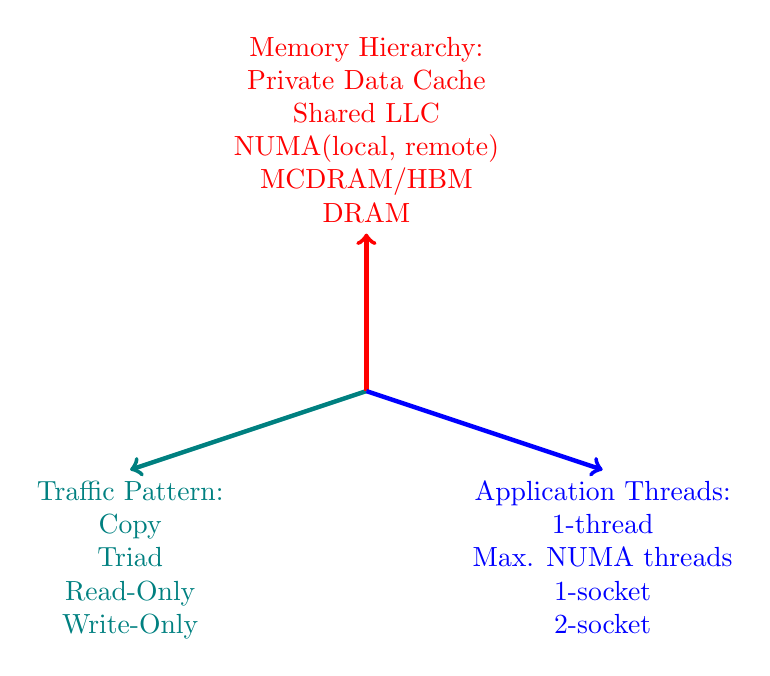
\begin{tikzpicture}
\draw[teal, ultra thick, ->] (0,1) -- (-3,0)node[align=center, below] {Traffic Pattern:\\Copy\\Triad\\Read-Only\\Write-Only};
\draw[red, ultra thick, ->] (0,1) -- (0,3)node[align=center, above] {Memory Hierarchy:\\Private Data Cache\\Shared LLC\\NUMA(local, remote)\\MCDRAM/HBM\\DRAM};
\draw[blue, ultra thick, ->] (0,1) -- (3,0)node[align=center, below] {Application Threads:\\1-thread\\Max. NUMA threads\\1-socket\\2-socket};
\end{tikzpicture}
\caption{Memory sub-system study} \label{figure:1}
\end{figure}

\subsection{Scope of Study}
This report aims to characterize the memory bandwidth and latency for the following 3 CPU architectures:
\begin{enumerate}
    \item AMD Rome (2$^{nd}$ generation EPYC Processors)
    \item Intel Cascade Lake (2$^{nd}$  generation Xeon Scalable Processors)
    \item Intel Ice Lake (3$^{rd}$  generation Xeon Scalable Processors)
\end{enumerate}
Since memory bandwidth and latency is a broad topic, we will limit the scope of this study to the following aspects --
\begin{enumerate}
\item More emphasis on DDR memory bandwidth followed by cache bandwidth and latency.
\item Synthetic kernels consisting of contiguous access pattern.
\end{enumerate}

In the following sections, we will describe the experiments setup and benchmark methodology. This is followed by providing the DRAM memory bandwidth results for different traffic patterns, thread configurations, type of store instructions and NUMA domain. Next, we will provide the cache bandwidth and latency results. 

\section{Experiments Setup}
\subsection{Hardware Platforms}
The details of the CPU configuration benchmarked in this study are listed in table-\ref{table:hw_platforms}. It is important to note that the CPU's have different memory channels, memory speed, number of cores etc. In the rest of the document, we will refer to the CPU platforms by their corresponding code-names.

\begin{table}[h!]
\centering
 \begin{tabular}{|l|c|c|c|} \hline
& AMD Epyc 7742 & Intel Xeon 8268 & Intel ICX XCC \\\hline
Code name & Rome & Cascade Lake (CLX) & Ice Lake (ICX) \\ \hline
Number of sockets & 2 & 2 & 2 \\ \hline
Number of cores per socket & 64 & 24 & 32 \\ \hline
Total number of cores & 128 & 48 & 64 \\ \hline
LLC per socket & 256 MB & 35.7 MB & 48 MB \\ \hline
Total memory & 264 GB & 197 GB & 264 GB \\ \hline
Memory type & DDR4 @ 3200 MT/s & DDR4 @ 2933 MT/s & DDR4 @ 3200 MT/s \\ \hline
Memory channels per socket & 8 & 6 & 8 \\ \hline
Theoretical Peak B/W per socket & 204.8 GB/s & 140.8 GB/s & 204.8 GB/s\\   \hline
Theoretical Peak B/W & 409.6 GB/s & 281.6 GB/s & 409.6 GB/s\\   \hline
\end{tabular}
\caption{Hardware Platforms}
\label{table:hw_platforms}
\end{table}

The theoretical peak memory bandwidth is calculated as: 
\begin{align*}
 Peak\: B/W\: (GB/s) = x\: GT/s\: \times\: 8 \:bytes\_per\_channel\: \times\:  n\: channels\_per\_socket \times m\: sockets
\end{align*}

\subsection{STREAM Benchmark}
STREAM is a widely used standard benchmark to characterize the memory performance. It consists of the following 4 kernels -- Copy, Scale, Add, Triad. The characteristics of these kernels are listed in table-\ref{table:stream_kernels}. As can be observed from the table, Scale and Add process the same number of bytes as Copy and Triad respectively and only differ in the floating-point operations. The differences in floating-point calculations is insignificant as these operations are memory-bound. Hence, we do not show the performance of these two kernels in the remaining part of the report.

To cover additional traffic patterns, we developed two more kernels representing 100\% read (Reduce) and 100\% write traffic (Fill). The Reduce kernel performs a vector reduction by an \textit{add} operator and the Fill kernel writes a constant scalar value to all elements of a buffer. The source code for these kernels can be accessed at the following internal GIT repository \url{https://gitlab.devtools.intel.com/vsripath/stream/}

\subsubsection{Target ISA}
The ISA used determines how many number of bytes are transferred to/from memory from/to CPU registers in a single vector instruction. AVX2 and AVX512F vector instructions operate on 256b and 512b wide CPU registers respectively and hence transfer 32B and 64B per load/store instruction respectively. STREAM benchmark is compiled with Intel C Compiler with the relevant flags to generate the optimal instruction generation for the target processor. The highest ISA supported on AMD Rome and Intel CLX, ICX is AVX2 and AVX512F respectively. Hence, AVX2 and AVX512F instructions are generated in the binary that is executed on AMD Rome and Intel CLX, ICX respectively. Refer to the makefile at the aforementioned GIT source repository for all the Compiler flags used in building the binaries used in this study.

\subsubsection{Cache Write Policy: vmovpd vs vmovntpd}
A CPU caches' write policy determines how and when the data in cache is written back to main memory. Usually, there are two write policies -- \textit{write-through and write-back}. Both AMD Rome and Intel CLX, ICX use \textit{write-back (WB)} cache policy. In WB policy, when the CPU modifies data, it's only updated in the cache and the write to the main memory is postponed until the cache line containing the updated data is evicted. Hence, a read-miss on a WB cache may require two memory accesses -- if modified, write the contents of the to-be evicted cache line to main memory and then fetch the requested data from main memory. For write-misses, they can be two approaches -- \textit{write-allocate, no-write allocate}. In \textit{write-allocate} policy, a store that misses the cache first fetches the cache line containing the data from main memory. And then when combined with the \textit{write-back} policy, results in an additional memory access to write the updated data back to main memory.

If we look at the STREAM kernels, we observe the following two characteristics --
\begin{itemize}
\item Full Cache Line update: There are no partial cache line modifications done by the kernels.
\item Non-Temporal Locality: The data that is written is never accessed/read again. Hence, there is no need to keep the data in cache.
\end{itemize}

Considering these aspects of STREAM kernels, we can observe that the \textit{write-allocate} policy introduces an unnecessary overhead of fetching the data to cache. This introduces additional constrains on memory bandwidth when all the cores are actively writing data to main memory. To alleviate this, we can use an alternative store instruction called \textit{non-temporal} store (vmovntpd) which by-passes the cache and directly writes to main memory.

In order to understand the impact of type of store instruction on memory bandwidth performance, STREAM benchmark is compiled in the following two configurations --
\begin{itemize}
\item Regular Stores: This configuration uses regular stores (vmovpd) that generates two memory accesses on a write-miss. We will refer to this configuration as Read-For-Ownership (RFO) in the rest of the report. RFO is a cache coherency operation specifying a read operation with intent to write to that memory address.
\item Non-Temporal (NT) Stores: This configuration uses the aforementioned vmovntpd instruction to write back directly to main memory without bringing the data into cache. We will refer to this configuration as NT in the rest of the report.
\end{itemize}

For the different STREAM kernels, we can come up with the following expected speed-up of NT over RFO --
\begin{itemize}
\item Copy: The Copy kernel has a total of 2 (1 read, 1 write) and 3 (2-reads, 1 write) memory-ops when using NT and regular stores respectively. Hence, the ideal speed-up of NT over RFO should be 1.5x.
\item Triad: The Triad kernel has a total of 3 (2 reads, 1 write) and 4 (3 reads, 1 write) memory-ops when using NT and regular stores. Hence, the ideal speed-up of NT over RFO should be 1.33x.
\item Reduce: The Reduce kernel has 0 write ops and so the performance should remain the same with both NT and regular stores.
\item Fill: The Fill kernel has only memory write ops and so the ideal speed-up of NT over RFO should be 2x.
\end{itemize}

\begin{table}[h!]
\centering
 \begin{tabular}{|l|l|c|c|c|c|c|}
 \hline
 Kernel & Op & \makecell{Bytes Read \\ (RFO)} & \makecell{Bytes Read \\ (NT)} & \makecell{Bytes \\Written} & FLOPs & \makecell{Ideal Speed-up\\ of NT over RFO} \\ \hline
 COPY & \(a[i] = b[i]\)& 16 & 8 & 8 & 0 & 1.5x\\ \hline
 SCALE & \(a[i] = scalar \times b[i]\) & 16 & 8 & 8 & 1 & 1.5x\\ \hline
 ADD & \(c[i] = a[i] + b[i]\) & 24 & 16 & 8 & 1 & 1.33x \\ \hline
 TRIAD & \(c[i] = a[i] + scalar \times b[i]\) & 24 & 16 & 8 & 2 & 1.33x \\ \hline
 REDUCE & \(sum += a[i]\) & 8 & 8 & 0 & 1 & 1x \\ \hline
 FILL & \(a[i] = constant\) & 8 & 0 & 8 & 0 & 2x \\  \hline
\end{tabular}
\caption{STREAM Kernels}
\label{table:stream_kernels}
\end{table}

\subsection{Intel Memory Latency Checker}For cache bandwidth and latency analysis, we rely on the more versatile  \href{https://software.intel.com/content/www/us/en/develop/articles/intelr-memory-latency-checker.html}{Intel Memory Latency Checker}.


\subsection{Runtime Settings}
Table-\ref{table:3} shows the run-time settings used for most of the results presented in this study. Where we depart from these settings, we will explicitly call out the changes in the corresponding section.

\begin{table}[h!]
\centering
\begin{tabular}{|c|c|c|c|}  \hline
 & AMD Rome 7742 & Intel Xeon 8268 & Intel ICX XCC \\ \hline
NUMA per socket & 4 & 1 & 1 \\ \hline
Operating System & \multicolumn{3}{c|}{CentOS Linux 7 (Core)} \\  \hline
Kernel & \multicolumn{3}{c|}{3.10.0-1127.18.2.el7.crt1.x86\_64} \\ \hline
CPU Turbo Boost & \multicolumn{3}{c|}{Enabled} \\  \hline
CPU Scaling Governor & \multicolumn{3}{c|}{userspace} \\  \hline
CPU Scaling Driver & \multicolumn{3}{c|}{acpi-cpufreq} \\  \hline
Transparent Huge Pages & \multicolumn{3}{c|}{Enabled} \\  \hline
Intel C Compiler & \multicolumn{3}{c|}{ICC 19.1.2.254 20200623} \\  \hline
Hyper-Threading & \multicolumn{3}{c|}{\makecell{Enabled in HW,\\but logical threads are not used in benchmarking}} \\
\hline
OpenMP Thread Affinity & \multicolumn{3}{c|}{KMP\_AFFINITY = \say{granularity=fine,compact,1,0}} \\ \hline
\end{tabular}
\caption{Runtime Settings}
\label{table:3}
\end{table}

\section{DRAM}
In the following sub-sections, we will look at the peak achieved memory bandwidth by different CPU's in 1-core, 1-socket and 2-socket configuration. We will also evaluate the scaling performance within a socket and the impact of NUMA domains and OpenMP thread to CPU core affinity as well. Each sub-section contains performance data to primarily answer the following two questions -- 

\begin{enumerate}
\item How does the different CPU architectures compare against each other?
\item What is the impact of using RFO and NT stores on a given architecture?
\end{enumerate}

\subsection{1-Core}

\begin{figure}[!ht]
    \centering
    \begin{subfigure}[!ht]{0.3\textwidth}
         \centering
         \includegraphics[width=\textwidth]{../mem_bw_core/mb_core_rfo}
         \caption{RFO}
         \label{figure:mem_bw_core_rfo}
    \end{subfigure}
    \begin{subfigure}[!ht]{0.3\textwidth}
         \centering
         \includegraphics[width=\textwidth]{../mem_bw_core/mb_core_nt}
         \caption{NT}
         \label{figure:mem_bw_core_nt}
    \end{subfigure}
    \begin{subfigure}[!ht]{0.3\textwidth}
         \centering
         \includegraphics[width=\textwidth]{../mem_bw_core/mb_core_nt_rfo}
         \caption{Speed-up of NT over RFO}
         \label{figure:mem_bw_core_nt_rfo}
    \end{subfigure}

    \caption{STREAM 1-Core DRAM bandwidth}
    \label{figure:mem_bw_core}
\end{figure}

\subsubsection{Peak Bandwidth with RFO}
Figure-\ref{figure:mem_bw_core_rfo} RFO observations:
\begin{enumerate}
\item Rome vs ICX: Even though these two processors have identical DRAM configuration, Rome delivers 15-40\% higher bandwidth for Copy, Triad and Reduce kernels. For the Fill kernel, Rome is better than ICX by 2x.
\item ICX vs CLX: Comparing gen-to-gen Xeon performance, there is a 20\% improvement for Triad and Reduce kernels, with Fill showing a slow-down of 64\%.
\item Table-\ref{table:mem_bw_core_rfo} summarizes the speed-up of all kernels.
\end{enumerate}

\begin{table}[h!]
\centering
\begin{tabular}{|c|c|c|c|c|c|c|}  \hline
Kernel&Rome&CLX&ICX & ICX/Rome & CLX/Rome & ICX/CLX \\ \hline 
Copy & 18.25 & 12.85 & 13.17  & 0.72 & 0.70 & 1.02 \\ \hline 
Triad & 20.73 & 13.42 & 16.27  & 0.78 & 0.65 & 1.21 \\ \hline 
Reduce & 19.40 & 13.30 & 16.77  & 0.86 & 0.69 & 1.26 \\ \hline 
Fill & 15.29 & 11.77 & 7.14  & 0.47 & 0.77 & 0.61 \\ \hline 
\end{tabular}

\caption{1-Core peak bandwidth: RFO}
\label{table:mem_bw_core_rfo}
\end{table}

\subsubsection{Peak Bandwidth with NT}

Figure-\ref{figure:mem_bw_core_nt} NT observations:
\begin{enumerate}
\item Rome vs ICX: Similar to the trend observed with RFO stores, Rome delivers higher bandwidth (33-50\%) for Copy, Triad and Reduce kernels. However, for the Fill kernel ICX beats Rome by 1.12x.
\item ICX vs CLX: ICX delivers significant performance gains of 2.4, 3.7x for Copy and Fill kernels. Triad and Reduce show 1.6x and 1.3x gains respectively.
\item Table-\ref{table:mem_bw_core_nt} summarizes the speed-up of all kernels.
\end{enumerate}


\begin{table}[h!]
\centering
\begin{tabular}{|c|c|c|c|c|c|c|}  \hline
Kernel&Rome&CLX&ICX & ICX/Rome & CLX/Rome & ICX/CLX \\ \hline 
Copy & 36.59 & 10.36 & 24.70  & 0.68 & 0.28 & 2.38 \\ \hline 
Triad & 31.48 & 13.06 & 20.95  & 0.67 & 0.41 & 1.60 \\ \hline 
Reduce & 22.49 & 12.78 & 16.76  & 0.75 & 0.57 & 1.31 \\ \hline 
Fill & 23.42 & 7.15 & 26.29  & 1.12 & 0.31 & 3.68 \\ \hline 
\end{tabular}

\caption{1-Core peak bandwidth: NT}
\label{table:mem_bw_core_nt}
\end{table}

\subsubsection{RFO vs. NT Stores}

Figure-\ref{figure:mem_bw_core_nt_rfo} observations:
\begin{enumerate}
\item Across the CPU's, the Reduce kernel performance remains identical between NT and RFO configurations since it has no writes to main memory.
\item Rome: As can be expected, NT stores show higher performance than using regular stores which generate RFO requests. Interestingly, the speed-up of Copy kernel with NT stores exceeds the expected speed-up.
\item CLX: None of the kernels shows gains with NT. This indicates that memory bandwidth is not the constraint when using 1 core because RFO generates more memory traffic than NT. This leads to the observation that when the system is not memory bandwidth constrained (as is the case here with 1-thread), the latency of NT stores is greater than regular stores. This could be due to the fact that the hardware prefetchers do a good job of fetching the write-miss requests with regular stores. In contrast, with NT stores the hardware prefetchers have no active role since the data is never to be brought into cache.
\item ICX: ICX delivers the expected speed-up of NT over regular stores for all the kernels. The Fill kernel speed-up of 3.5x exceeds the ideal speed-up of 2x.
\end{enumerate}


\subsection{1-Socket}
\begin{figure}[!ht]
    \centering
    \includegraphics[width=0.24\textwidth]{../mem_bw_scale/mb_scale_compact_Copy_rfo}
    \includegraphics[width=0.24\textwidth]{../mem_bw_scale/mb_scale_compact_Triad_rfo}
    \includegraphics[width=0.24\textwidth]{../mem_bw_scale/mb_scale_compact_Reduce_rfo}
    \includegraphics[width=0.24\textwidth]{../mem_bw_scale/mb_scale_compact_Fill_rfo}
    \caption{STREAM 1-Socket DRAM bandwidth scaling with RFO and Compact pinning}
    \label{figure:mem_bw_scale_compact_rfo}
\end{figure}

For these experiments, Rome is configured to be in 4 NUMA domains Per Socket (NPS) mode whereas ICX and CLX are configured to have 1 NPS. Also, OpenMP threads are pinned to cores that are closer first i.e., compact mode. We will explore the performance impact of distributed pinning in the next section.

\subsubsection{Peak Bandwidth and Scaling with RFO}
Figure-\ref{figure:mem_bw_scale_compact_rfo} observations:
\begin{itemize}
\item Peak Bandwidth: Using all the cores in the socket
\begin{itemize}
\item Rome vs ICX: Contrary to 1-core performance, ICX beats Rome for all kernels using RFO stores.
\item Rome vs CLX: Rome delivers superior performance for all kernels.
\item ICX vs CLX: Comparing gen-to-gen Xeon performance, ICX delivers significant performance improvements over CLX for all kernels.
\item Table-\ref{table:mem_bw_socket_rfo} shows the speed-up of all kernels.
\end{itemize}
\item Scaling Performance: 
\begin{itemize}
\item Rome: Across the 4 kernels, Rome exhibits similar scaling performance pattern. Since Rome contains 64 cores per socket partitioned into 4 NUMA domains, each NUMA domain contains 16 cores. The data in the figure shows that the performance remains similar from 1 to 16 threads i.e., when threads are populated in NUMA domain-0. After that, the performance increases linearly with thread count and the gains from 16 to 64 threads show ideal scaling behavior.
\item CLX, ICX: In contrast to Rome, both CLX and ICX reach close to peak bandwidth using much less number of threads. In addition, CLX shows higher performance at some thread counts for Fill kernel.
\end{itemize}
\end{itemize}

\begin{table}[h!]
\centering
\begin{tabular}{|c|c|c|c|c|c|c|}  \hline
Kernel&Rome&CLX&ICX & ICX/Rome & CLX/Rome & ICX/CLX \\ \hline 
Copy & 101.91 & 71.92 & 151.72  & 1.49 & 0.71 & 2.11 \\ \hline 
Triad & 111.82 & 81.35 & 155.98  & 1.39 & 0.73 & 1.92 \\ \hline 
Reduce & 122.14 & 115.73 & 159.14  & 1.30 & 0.95 & 1.38 \\ \hline 
Fill & 86.25 & 51.38 & 153.83  & 1.78 & 0.60 & 2.99 \\ \hline 
\end{tabular}

\caption{1-Socket peak bandwidth: RFO}
\label{table:mem_bw_socket_rfo}
\end{table}

\subsubsection{Peak Bandwidth and Scaling with NT}

\begin{figure}[!ht]
    \centering
    \includegraphics[width=0.24\textwidth]{../mem_bw_scale/mb_scale_compact_Copy_nt}
    \includegraphics[width=0.24\textwidth]{../mem_bw_scale/mb_scale_compact_Triad_nt}
    \includegraphics[width=0.24\textwidth]{../mem_bw_scale/mb_scale_compact_Reduce_nt}
    \includegraphics[width=0.24\textwidth]{../mem_bw_scale/mb_scale_compact_Fill_nt}
    \caption{STREAM 1-Socket DRAM bandwidth scaling with NT Stores and Compact pinning}
    \label{figure:mem_bw_scale_compact_nt}
\end{figure}

Figure-\ref{figure:mem_bw_scale_compact_nt} observations:
\begin{itemize}
\item Peak Bandwidth: Using all the cores in the socket
\begin{itemize}
\item Rome vs ICX: Contrary to RFO, ICX delivers similar performance as Rome, with the Fill kernel showing 7\% slow-down.
\item Rome vs CLX: Rome delivers superior performance for all kernels.
\item ICX vs CLX: Comparing gen-to-gen Xeon performance, ICX delivers 42-79\% performance improvements over CLX depending on STREAM kernel.
\item Table-\ref{table:mem_bw_socket_nt} shows the speed-up of all kernels.
\end{itemize}
\item Scaling Performance: The scaling profile looks similar to RFO except for the following exceptions --
\begin{itemize}
\item Rome: The Fill kernel shows gains with thread count starting at 8 instead of 16 as observed with RFO stores.
\item CLX, ICX: On ICX, the Fill kernel loses performance when using all the threads in the socket. This results in reduction of about 10\% peak bandwidth for this kernel.
\end{itemize}
\end{itemize}

\begin{table}[h!]
\centering
\begin{tabular}{|c|c|c|c|c|c|c|}  \hline
Kernel&Rome&CLX&ICX & ICX/Rome & CLX/Rome & ICX/CLX \\ \hline 
Copy & 159.39 & 107.55 & 160.40  & 1.01 & 0.67 & 1.49 \\ \hline 
Triad & 156.29 & 110.45 & 161.14  & 1.03 & 0.71 & 1.46 \\ \hline 
Reduce & 171.97 & 123.45 & 175.31  & 1.02 & 0.72 & 1.42 \\ \hline 
Fill & 157.72 & 81.99 & 146.77  & 0.93 & 0.52 & 1.79 \\ \hline 
\end{tabular}

\caption{1-Socket peak bandwidth: NT}
\label{table:mem_bw_socket_nt}
\end{table}


\subsubsection{RFO vs. NT Stores}

\begin{figure}[!ht]
    \centering
    \includegraphics[width=0.24\textwidth]{../mem_bw_scale/mb_scale_compact_Copy_nt_rfo}
    \includegraphics[width=0.24\textwidth]{../mem_bw_scale/mb_scale_compact_Triad_nt_rfo}
    \includegraphics[width=0.24\textwidth]{../mem_bw_scale/mb_scale_compact_Reduce_nt_rfo}
    \includegraphics[width=0.24\textwidth]{../mem_bw_scale/mb_scale_compact_Fill_nt_rfo}
    \caption{STREAM 1-Socket DRAM bandwidth scaling, speed-up of NT over RFO Stores}
    \label{figure:mem_bw_scale_compact_nt_rfo}
\end{figure}

\begin{enumerate}
\item Copy: As mentioned in table-\ref{table:stream_kernels}, the ideal speed-up of NT over RFO for Copy kernel should be 1.5x. Rome matches with the expected ideal speed-up. CLX reaches the 1.5x speed-up at higher thread count. On ICX, the gains of using NT stores vanishes as thread count increases. Also, to be noted is that CLX and ICX exhibit opposing scaling curve.
\item Triad: The ideal speed-up of NT over RFO for Triad should be 1.33x. Rome exhibits the ideal speed-up. CLX shows expected gains at higher thread counts, whereas ICX shows maximum gains of about 1.3x at lower threads counts with NT stores.
\item Reduce: The performance of Reduce kernel should remain identical with both NT and regular stores. However, the Reduce kernel on Rome shows up to 40\% performance gains with NT stores. Deeper investigation of this kernel code generation revealed that the Intel compiler does aggressive unrolling when using regular stores. This results in more in-flight loads and appears to be the root-cause for the slowdown with regular stores. Interestingly, even though the Intel Compiler does the same aggressive unrolling with regular stores on CLX and ICX, these two architectures seems to be more resilient to additional in-flight loads and do not result in lower performance.
\item Fill: The ideal speed-up of NT over RFO should be 2x. Rome reaches the expected gains once the thread count is greater than the number of cores of NUMA domain. CLX and ICX exhibit different behavior for this kernel with ICX continuing the trend of losing gains of using NT over regular stores as thread count increases.
\end{enumerate}


\subsubsection{Compact vs Distributed Pinning}
The experiments with thread affinity settings make for an interesting performance study only when there are multiple NUMA domains in a socket. Since only Rome is configured to have 4 NUMA domains per socket in our setup, we will limit these experiments to Rome architecture. As mentioned earlier, Compact pinning refers to thread affinity scheme where OpenMP threads are pinned to cores that are closer to each other. In distributed pinning scheme, we affinitize the OpenMP threads to spread across the NUMA domains first. For e.g, with 4 threads this translates to using a single core on each of the 4 NUMA domains in a socket.

\begin{figure}[!ht]
    \centering
    \includegraphics[width=0.45\textwidth]{../mem_bw_scale/Rome_scale_affinity_rfo}
    \includegraphics[width=0.45\textwidth]{../mem_bw_scale/Rome_scale_affinity_nt}
    \caption{STREAM 1-Socket DRAM bandwidth: Compact vs Distributed Pinning}
    \label{figure:mem_bw_scale_affinity_rfo_nt}
\end{figure}

Figure-\ref{figure:mem_bw_scale_affinity_rfo_nt} observations:
\begin{itemize}
\item For both RFO and NT, close to peak bandwidth is achieved with fewer threads in distributed pinning when compared to compact mode. This make sense since in NPS-4 mode, the 8 memory channels are partitioned to the 4 NUMA domains with each NUMA domain accessing DRAM through 2 channels. Hence, with 8 threads all memory channels are actively used in distributed pinning.
\item RFO: The Reduce kernel with distributed affinity reaches peak bandwidth at fewer threads and then loses performance when using all the cores in the socket.
\item NT: When compared to the rest of the kernels, the Fill kernel in distributed pinning shows much less achieved bandwidth. Once the number of threads reaches more than 32, the performance is only marginally better than compact pinning.
\end{itemize}

\subsection{2-Socket} \label{2-socket}
\begin{figure}[!ht]
    \centering
    \begin{subfigure}[!ht]{0.3\textwidth}
         \centering
         \includegraphics[width=\textwidth]{../mem_bw_node/mb_node_rfo}
         \caption{RFO}
         \label{figure:mem_bw_node_rfo}
    \end{subfigure}
    \begin{subfigure}[!ht]{0.3\textwidth}
         \centering
         \includegraphics[width=\textwidth]{../mem_bw_node/mb_node_nt}
         \caption{NT}
         \label{figure:mem_bw_node_nt}
    \end{subfigure}
    \begin{subfigure}[!ht]{0.3\textwidth}
         \centering
         \includegraphics[width=\textwidth]{../mem_bw_node/mb_node_nt_rfo}
         \caption{Speed-up of NT over RFO}
         \label{figure:mem_bw_node_nt_rfo}
    \end{subfigure}

    \caption{STREAM 2-socket DRAM bandwidth}
    \label{figure:mem_bw_node}
\end{figure}

Figure-\ref{figure:mem_bw_node} shows the peak achieved bandwidth when all cores in a 2 socket system are accessing data to/from DRAM. Table-\ref{table:mem_bw_node_rfo}, \ref{table:mem_bw_node_nt} show the corresponding speed-up for each of the architecture with RFO and NT stores respectively. Since each socket has it's own set of memory controllers, DRAM bandwidth for 2-socket scales by a factor of 2 compared to 1-socket performance. There are no unique observations when it comes to 2-socket data and all the points made in the 1-socket section are valid here as well.

\subsubsection{Peak Bandwidth with RFO}
\begin{table}[h!]
\centering
\begin{tabular}{|c|c|c|c|c|c|c|}  \hline
Kernel&Rome&CLX&ICX & ICX/Rome & CLX/Rome & ICX/CLX \\ \hline 
Copy & 207.04 & 144.30 & 305.52  & 1.48 & 0.70 & 2.12 \\ \hline 
Triad & 224.69 & 161.42 & 313.66  & 1.40 & 0.72 & 1.94 \\ \hline 
Reduce & 193.15 & 228.17 & 307.77  & 1.59 & 1.18 & 1.35 \\ \hline 
Fill & 209.83 & 105.40 & 276.74  & 1.32 & 0.50 & 2.63 \\ \hline 
\end{tabular}

\caption{2-socket peak bandwidth: RFO}
\label{table:mem_bw_node_rfo}
\end{table}

\subsubsection{Peak Bandwidth with NT}
\begin{table}[h!]
\centering
\begin{tabular}{|c|c|c|c|c|c|c|}  \hline
Kernel&Rome&CLX&ICX & ICX/Rome & CLX/Rome & ICX/CLX \\ \hline 
Copy & 317.77 & 198.35 & 321.62  & 1.01 & 0.62 & 1.62 \\ \hline 
Triad & 311.98 & 217.81 & 324.89  & 1.04 & 0.70 & 1.49 \\ \hline 
Reduce & 341.00 & 244.26 & 345.71  & 1.01 & 0.72 & 1.42 \\ \hline 
Fill & 315.62 & 152.32 & 273.78  & 0.87 & 0.48 & 1.80 \\ \hline 
\end{tabular}

\caption{2-socket peak bandwidth: NT}
\label{table:mem_bw_node_nt}
\end{table}

Figure-\ref{figure:mem_bw_node} observations:
   \begin{itemize}
   \item RFO: See figure-\ref{figure:mem_bw_node_rfo}
      \begin{itemize}
         \item Rome vs ICX: ICX delivers 40-70\% higher performance (depending on kernel type) than Rome.
         \item Rome vs CLX: Rome delivers higher performance (38-80\%) than CLX with the exception of Reduce kernel.
         \item ICX vs CLX: Comparing gen-to-gen Xeon performance, ICX delivers significant performance improvements of 1.35x to 2.6x over CLX depending on STREAM kernel.
   \end{itemize}

   \item NT: See figure-\ref{figure:mem_bw_node_nt}
      \begin{itemize}
         \item Rome vs ICX: The performance of Copy and Reduce kernels are identical on Rome and CLX. ICX shows 4\% better performance for Triad whereas Rome is 15\% better ICX for Fill kernel. 
         \item Rome vs CLX: Rome delivers superior performance (40-100\%) depending on STREAM kernel.
         \item ICX vs CLX: ICX shows 1.4-1.8x higher performance depending on STREAM kernel.
      \end{itemize}
   \end{itemize}

\subsection{NUMA}
In this section, we will explore the performance impact of explicitly pinning memory to a specific NUMA domain. We achieve this by doing the following: 
\begin{enumerate}
\item NUMA Placement: Explicitly specify a single NUMA domain using \textit{numactl}. This forces all the memory accesses to go to that NUMA domain.
\item Threads Placement: For both 1-core and 1-socket (utilizing all the cores in a socket), we explicitly pin the OpenMP threads to socket-0 cores. 
\item The combination of the above two enables us to evaluate the cross-socket interconnect (Intel UPI, AMD Infinity Fabric) bandwidth as well.
\item Since Rome and CLX, ICX are setup in different NPS modes, it is not a fair one-to-one comparison. Rather, it should be seen as what are the trade-offs of using one mode on given architecture on application performance.
\end{enumerate}
 
\begin{figure}[!ht]
    \centering
    \includegraphics[width=0.3\textwidth]{../mem_bw_numa/Rome_numa_nps4_compact_rfo}
    \includegraphics[width=0.3\textwidth]{../mem_bw_numa/ICX_numa_nps1_compact_rfo}
    \includegraphics[width=0.3\textwidth]{../mem_bw_numa/CLX_numa_nps1_compact_rfo}
    \caption{STREAM 1-Core, 1-Socket NUMA bandwidth with RFO}
    \label{figure:mem_bw_numa_rfo}
\end{figure}


\subsubsection{1-Core, 1-Socket:}
Figure-\ref{figure:mem_bw_numa_rfo} shows the performance of STREAM kernels with regular stores using different NUMA domains. There isn't much difference between RFO and NT stores with respect to NUMA, so we will just focus our discussion on the impact of NUMA. Figure-\ref{figure:mem_bw_numa_nt} in the appendix section shows the performance with NT stores.
\begin{itemize}
\item Rome:
\begin{itemize}
\item Local vs Remote NUMA: Since Rome is setup in NPS-4 mode, it has 4 NUMA domain domains per socket (0-3) and a total of 8 NUMA domains in a 2-socket system. This naturally translates to higher bandwidth for memory accesses going to local NUMA domains in socket-0 i.e., NUMA domain 0 to 3. With NUMA domain 4 to 7, the memory requests have to cross the socket over the on-chip interconnect and hence leads to lower performance.
\item Local NUMA: In NPS-4, memory accesses going to each NUMA domain are interleaved across only 2 memory channels (4 NUMA domains $\times$ 2 channels = 8 channels), this leads to substantially lower memory bandwidth even when using all cores in a socket. This can be observed by comparing the 1-socket performance in figure-\ref{figure:mem_bw_numa_rfo} with figure-\ref{figure:mem_bw_scale_compact_rfo} where memory is distributed across all NUMA domain in a socket.
\end{itemize}

\item CLX, ICX:
\begin{itemize}
\item Local vs Remote NUMA: Comparing gen-to-gen, the cross-socket memory bandwidth shows more than 2x gains in ICX.
\item Local NUMA: Since both CLX and ICX are in NPS-1 mode, memory accesses use all the available channels in a socket. Hence, the 1-socket performance in figure-\ref{figure:mem_bw_numa_rfo} is identical to figure-\ref{figure:mem_bw_scale_compact_rfo}
\end{itemize}
\end{itemize}


\clearpage
\subsection{Sub-NUMA Clustering} \label{snc}
\subsubsection{ICX: SNC-1, 2, 4}

\begin{figure}[!hb]
    \centering
    \begin{subfigure}[!hb]{0.3\textwidth}
         \centering
         \includegraphics[width=\textwidth]{../icx-32c-snc/mem_bw_core/mb_core_rfo}
         \caption{RFO}
         \label{figure:mem_bw_core_rfo_icx_snc}
    \end{subfigure}
    \begin{subfigure}[!hb]{0.3\textwidth}
         \centering
         \includegraphics[width=\textwidth]{../icx-32c-snc/mem_bw_core/mb_core_nt}
         \caption{NT}
         \label{figure:mem_bw_core_nt_icx_snc}
    \end{subfigure}
    \begin{subfigure}[!hb]{0.3\textwidth}
         \centering
         \includegraphics[width=\textwidth]{../icx-32c-snc/mem_bw_core/mb_core_nt_rfo}
         \caption{Speed-up of NT over RFO}
         \label{figure:mem_bw_core_nt_rfo_icx_snc}
    \end{subfigure}

    \caption{STREAM ICX 1-Core DRAM bandwidth: SNC modes}
    \label{figure:mem_bw_core_icx_snc}
\end{figure}

\begin{figure}[!hb]
    \centering
    \begin{subfigure}[!hb]{0.3\textwidth}
         \centering
         \includegraphics[width=\textwidth]{../icx-32c-snc/mem_bw_node/mb_node_rfo}
         \caption{RFO}
         \label{figure:mem_bw_node_rfo_icx_snc}
    \end{subfigure}
    \begin{subfigure}[!hb]{0.3\textwidth}
         \centering
         \includegraphics[width=\textwidth]{../icx-32c-snc/mem_bw_node/mb_node_nt}
         \caption{NT}
         \label{figure:mem_bw_node_nt_icx_snc}
    \end{subfigure}
    \begin{subfigure}[!hb]{0.3\textwidth}
         \centering
         \includegraphics[width=\textwidth]{../icx-32c-snc/mem_bw_node/mb_node_nt_rfo}
         \caption{Speed-up of NT over RFO}
         \label{figure:mem_bw_node_nt_rfo_icx_snc}
    \end{subfigure}

    \caption{STREAM ICX 2-Socket DRAM bandwidth: SNC modes}
    \label{figure:mem_bw_node_icx_snc}
\end{figure}


\begin{figure}[!hb]
    \centering
    \includegraphics[width=0.24\textwidth]{../icx-32c-snc/mem_bw_scale/mb_scale_compact_Copy_rfo}
    \includegraphics[width=0.24\textwidth]{../icx-32c-snc/mem_bw_scale/mb_scale_compact_Triad_rfo}
    \includegraphics[width=0.24\textwidth]{../icx-32c-snc/mem_bw_scale/mb_scale_compact_Reduce_rfo}
    \includegraphics[width=0.24\textwidth]{../icx-32c-snc/mem_bw_scale/mb_scale_compact_Fill_rfo}
    \caption{STREAM 1-Socket DRAM bandwidth scaling with RFO and Compact pinning: SNC modes}
    \label{figure:mem_bw_scale_compact_rfo_icx_snc}
\end{figure}

\begin{figure}[!hb]
    \centering
    \includegraphics[width=0.24\textwidth]{../icx-32c-snc/mem_bw_scale/mb_scale_special_Copy_rfo}
    \includegraphics[width=0.24\textwidth]{../icx-32c-snc/mem_bw_scale/mb_scale_special_Triad_rfo}
    \includegraphics[width=0.24\textwidth]{../icx-32c-snc/mem_bw_scale/mb_scale_special_Reduce_rfo}
    \includegraphics[width=0.24\textwidth]{../icx-32c-snc/mem_bw_scale/mb_scale_special_Fill_rfo}
    \caption{STREAM 1-Socket DRAM bandwidth scaling with RFO with specific affinity: SNC modes}
    \label{figure:mem_bw_scale_special_rfo_icx_snc}
\end{figure}

\begin{figure}[!hb]
    \centering
    \includegraphics[width=0.3\textwidth]{../icx-32c-snc/mem_bw_numa/SNC-1_numa_nps1_compact_rfo}
    \includegraphics[width=0.3\textwidth]{../icx-32c-snc/mem_bw_numa/SNC-2_numa_nps2_compact_rfo}
    \includegraphics[width=0.3\textwidth]{../icx-32c-snc/mem_bw_numa/SNC-4_numa_nps4_compact_rfo}
    \caption{STREAM 1-Core, 1-Socket NUMA bandwidth with RFO: SNC modes}
    \label{figure:mem_bw_numa_rfo_icx_snc}
\end{figure}

\begin{table}[!hb]
\centering
\begin{tabular}{|c|c|c|c|c|c|c|}  \hline
Kernel&SNC-1&SNC-2&SNC-4 & SNC-4/SNC-1 & SNC-2/SNC-1 & SNC-4/SNC-2 \\ \hline 
Copy & 13.17 & 13.99 & 13.99  & 1.06 & 1.06 & 1.00 \\ \hline 
Triad & 16.27 & 16.45 & 15.69  & 0.96 & 1.01 & 0.95 \\ \hline 
Reduce & 16.77 & 16.75 & 17.28  & 1.03 & 1.00 & 1.03 \\ \hline 
Fill & 7.14 & 7.52 & 7.66  & 1.07 & 1.05 & 1.02 \\ \hline 
\end{tabular}

\caption{ICX 1-Core peak bandwidth: RFO with SNC modes}
\label{table:mem_bw_core_rfo_icx_snc}
\end{table}
\begin{table}[!hb]
\centering
\begin{tabular}{|c|c|c|c|c|c|c|}  \hline
Kernel&SNC-1&SNC-2&SNC-4 & SNC-4/SNC-1 & SNC-2/SNC-1 & SNC-4/SNC-2 \\ \hline 
Copy & 24.70 & 25.50 & 23.16  & 0.94 & 1.03 & 0.91 \\ \hline 
Triad & 20.95 & 23.05 & 20.63  & 0.98 & 1.10 & 0.90 \\ \hline 
Reduce & 16.76 & 16.73 & 17.38  & 1.04 & 1.00 & 1.04 \\ \hline 
Fill & 26.29 & 29.81 & 31.62  & 1.20 & 1.13 & 1.06 \\ \hline 
\end{tabular}

\caption{ICX 1-Core peak bandwidth: NT with SNC modes}
\label{table:mem_bw_core_nt_icx_snc}
\end{table}
\begin{table}[!hb]
\centering
\begin{tabular}{|c|c|c|c|c|c|c|}  \hline
Kernel&SNC-1&SNC-2&SNC-4 & SNC-4/SNC-1 & SNC-2/SNC-1 & SNC-4/SNC-2 \\ \hline 
Copy & 305.52 & 303.83 & 290.05  & 0.95 & 0.99 & 0.95 \\ \hline 
Triad & 313.66 & 312.04 & 306.90  & 0.98 & 0.99 & 0.98 \\ \hline 
Reduce & 307.77 & 317.58 & 331.93  & 1.08 & 1.03 & 1.05 \\ \hline 
Fill & 276.74 & 274.89 & 283.67  & 1.03 & 0.99 & 1.03 \\ \hline 
\end{tabular}

\caption{ICX 2-Socket peak bandwidth: RFO with SNC modes}
\label{table:mem_bw_node_rfo_icx_snc}
\end{table}
\begin{table}[!hb]
\centering
\begin{tabular}{|c|c|c|c|c|c|c|}  \hline
Kernel&SNC-1&SNC-2&SNC-4 & SNC-4/SNC-1 & SNC-2/SNC-1 & SNC-4/SNC-2 \\ \hline 
Copy & 321.62 & 326.42 & 332.79  & 1.03 & 1.01 & 1.02 \\ \hline 
Triad & 324.89 & 330.86 & 338.79  & 1.04 & 1.02 & 1.02 \\ \hline 
Reduce & 345.71 & 361.04 & 357.46  & 1.03 & 1.04 & 0.99 \\ \hline 
Fill & 273.78 & 277.03 & 278.62  & 1.02 & 1.01 & 1.01 \\ \hline 
\end{tabular}

\caption{ICX 2-Socket peak bandwidth: NT with SNC modes}
\label{table:mem_bw_node_nt_icx_snc}
\end{table}



\paragraph{Summary}
\begin{itemize}
\item 1-Core, 2-Socket Memory Bandwidth: There are only marginal gains of using SNC on DRAM bandwidth.
\item NUMA: Since NUMA cluster is bound to fewer memory channels in SNC-2, 4 modes, the local and remote NUMA bandwidth is much lower compared to SNC-1 mode.
\end{itemize}
\clearpage
\subsubsection{CLX: SNC-1, 2}

\begin{figure}[!hb]
    \centering
    \begin{subfigure}[!hb]{0.3\textwidth}
         \centering
         \includegraphics[width=\textwidth]{../clx-8280l-snc/mem_bw_core/mb_core_rfo}
         \caption{RFO}
         \label{figure:mem_bw_core_rfo_clx_snc}
    \end{subfigure}
    \begin{subfigure}[!hb]{0.3\textwidth}
         \centering
         \includegraphics[width=\textwidth]{../clx-8280l-snc/mem_bw_core/mb_core_nt}
         \caption{NT}
         \label{figure:mem_bw_core_nt_clx_snc}
    \end{subfigure}
    \begin{subfigure}[!hb]{0.3\textwidth}
         \centering
         \includegraphics[width=\textwidth]{../clx-8280l-snc/mem_bw_core/mb_core_nt_rfo}
         \caption{Speed-up of NT over RFO}
         \label{figure:mem_bw_core_nt_rfo_clx_snc}
    \end{subfigure}

    \caption{STREAM CLX 1-Core DRAM bandwidth: SNC modes}
    \label{figure:mem_bw_core_clx_snc}
\end{figure}

\begin{figure}[!hb]
    \centering
    \begin{subfigure}[!hb]{0.3\textwidth}
         \centering
         \includegraphics[width=\textwidth]{../clx-8280l-snc/mem_bw_node/mb_node_rfo}
         \caption{RFO}
         \label{figure:mem_bw_node_rfo_clx_snc}
    \end{subfigure}
    \begin{subfigure}[!hb]{0.3\textwidth}
         \centering
         \includegraphics[width=\textwidth]{../clx-8280l-snc/mem_bw_node/mb_node_nt}
         \caption{NT}
         \label{figure:mem_bw_node_nt_clx_snc}
    \end{subfigure}
    \begin{subfigure}[!hb]{0.3\textwidth}
         \centering
         \includegraphics[width=\textwidth]{../clx-8280l-snc/mem_bw_node/mb_node_nt_rfo}
         \caption{Speed-up of NT over RFO}
         \label{figure:mem_bw_node_nt_rfo_clx_snc}
    \end{subfigure}

    \caption{STREAM CLX 2-Socket DRAM bandwidth: SNC modes}
    \label{figure:mem_bw_node_clx_snc}
\end{figure}


\begin{figure}[!hb]
    \centering
    \includegraphics[width=0.24\textwidth]{../clx-8280l-snc/mem_bw_scale/mb_scale_compact_Copy_rfo}
    \includegraphics[width=0.24\textwidth]{../clx-8280l-snc/mem_bw_scale/mb_scale_compact_Triad_rfo}
    \includegraphics[width=0.24\textwidth]{../clx-8280l-snc/mem_bw_scale/mb_scale_compact_Reduce_rfo}
    \includegraphics[width=0.24\textwidth]{../clx-8280l-snc/mem_bw_scale/mb_scale_compact_Fill_rfo}
    \caption{STREAM 1-Socket DRAM bandwidth scaling with RFO and Compact pinning: SNC modes}
    \label{figure:mem_bw_scale_compact_rfo_clx_snc}
\end{figure}

\begin{figure}[!hb]
    \centering
    \includegraphics[width=0.24\textwidth]{../clx-8280l-snc/mem_bw_scale/mb_scale_special_Copy_rfo}
    \includegraphics[width=0.24\textwidth]{../clx-8280l-snc/mem_bw_scale/mb_scale_special_Triad_rfo}
    \includegraphics[width=0.24\textwidth]{../clx-8280l-snc/mem_bw_scale/mb_scale_special_Reduce_rfo}
    \includegraphics[width=0.24\textwidth]{../clx-8280l-snc/mem_bw_scale/mb_scale_special_Fill_rfo}
    \caption{STREAM 1-Socket DRAM bandwidth scaling with RFO with specific affinity: SNC modes}
    \label{figure:mem_bw_scale_special_rfo_clx_snc}
\end{figure}

\begin{figure}[!hb]
    \centering
    \includegraphics[width=0.3\textwidth]{../clx-8280l-snc/mem_bw_numa/SNC-1_numa_nps1_compact_rfo}
    \includegraphics[width=0.3\textwidth]{../clx-8280l-snc/mem_bw_numa/SNC-2_numa_nps2_compact_rfo}
    \caption{STREAM 1-Core, 1-Socket NUMA bandwidth with RFO: SNC modes}
    \label{figure:mem_bw_numa_rfo_clx_snc}
\end{figure}

\begin{table}[!hb]
\centering
\begin{tabular}{|c|c|c|c|c|c|c|}  \hline
Kernel&SNC-1&SNC-2 & SNC-2/SNC-1 & SNC-1/SNC-1 & SNC-2/SNC-1 \\ \hline 
Copy & 12.93 & 14.15  & 1.09 & 1.00 & 1.09 \\ \hline 
Triad & 13.65 & 14.39  & 1.05 & 1.00 & 1.05 \\ \hline 
Reduce & 13.63 & 15.96  & 1.17 & 1.00 & 1.17 \\ \hline 
Fill & 11.75 & 12.83  & 1.09 & 1.00 & 1.09 \\ \hline 
\end{tabular}

\caption{CLX 1-Core peak bandwidth: RFO with SNC modes}
\label{table:mem_bw_core_rfo_clx_snc}
\end{table}
\begin{table}[!hb]
\centering
\begin{tabular}{|c|c|c|c|c|c|c|}  \hline
Kernel&SNC-1&SNC-2 & SNC-2/SNC-1 & SNC-1/SNC-1 & SNC-2/SNC-1 \\ \hline 
Copy & 10.49 & 11.02  & 1.05 & 1.00 & 1.05 \\ \hline 
Triad & 13.29 & 13.54  & 1.02 & 1.00 & 1.02 \\ \hline 
Reduce & 13.51 & 15.98  & 1.18 & 1.00 & 1.18 \\ \hline 
Fill & 7.23 & 7.67  & 1.06 & 1.00 & 1.06 \\ \hline 
\end{tabular}

\caption{CLX 1-Core peak bandwidth: NT with SNC modes}
\label{table:mem_bw_core_nt_clx_snc}
\end{table}
\begin{table}[!hb]
\centering
\begin{tabular}{|c|c|c|c|c|c|c|}  \hline
Kernel&SNC-1&SNC-2 & SNC-2/SNC-1 & SNC-1/SNC-1 & SNC-2/SNC-1 \\ \hline 
Copy & 141.11 & 144.28  & 1.02 & 1.00 & 1.02 \\ \hline 
Triad & 157.13 & 159.37  & 1.01 & 1.00 & 1.01 \\ \hline 
Reduce & 208.37 & 223.97  & 1.07 & 1.00 & 1.07 \\ \hline 
Fill & 100.90 & 106.81  & 1.06 & 1.00 & 1.06 \\ \hline 
\end{tabular}

\caption{CLX 2-Socket peak bandwidth: RFO with SNC modes}
\label{table:mem_bw_node_rfo_clx_snc}
\end{table}
\begin{table}[!hb]
\centering
\begin{tabular}{|c|c|c|c|c|c|c|}  \hline
Kernel&SNC-1&SNC-2 & SNC-2/SNC-1 & SNC-1/SNC-1 & SNC-2/SNC-1 \\ \hline 
Copy & 203.36 & 209.63  & 1.03 & 1.00 & 1.03 \\ \hline 
Triad & 215.35 & 215.68  & 1.00 & 1.00 & 1.00 \\ \hline 
Reduce & 243.25 & 247.07  & 1.02 & 1.00 & 1.02 \\ \hline 
Fill & 156.55 & 162.02  & 1.03 & 1.00 & 1.03 \\ \hline 
\end{tabular}

\caption{CLX 2-Socket peak bandwidth: NT with SNC modes}
\label{table:mem_bw_node_nt_clx_snc}
\end{table}


\clearpage
\section{CPU Caches}
Table-\ref{table:cache_subsystem} shows the cache hierarchy of AMD Rome and Intel CLX, ICX systems. We use Intel MLC to evaluate the cache performance on the target systems.\\
For latency measurements, the workload type is 100\% dependent reads with random access within a 512 KiB chunk. The dependent reads helps prevent pipelining, random access beats the hardware prefetchers and the 512 KiB chunk minimizes the TLB penalties.
\begin{table}[h!]
\centering
 \begin{tabular}{|l|c|c|c|} \hline
& AMD Epyc 7742 & Intel Xeon 8268 & Intel ICX XCC \\\hline
Code name & Rome & Cascade Lake (CLX) & Ice Lake (ICX) \\ \hline
Number of sockets & 2 & 2 & 2 \\ \hline
Number of cores per socket & 32 & 24 & 32 \\ \hline
Total number of cores & 64 & 48 & 64 \\ \hline
L1 Cache & \makecell{32 KiB\\(8-way private)} & \makecell{32 KiB\\(8-way private)} & \makecell{48 KiB\\(12-way private)}\\ \hline
L2 Cache & \makecell{512 KiB\\(8-way private)} & \makecell{1024 KiB\\(16-way private)} & \makecell{1280 KiB\\(20-way private)} \\ \hline
L3 Cache slice per core & 4 MiB & 1.5 MiB & 1.5 MiB \\ \hline
L3 Cache per socket & \makecell{256 MiB\\(16-way shared)} & \makecell{35.7 MiB\\(11-way shared)} & \makecell{48 MiB\\(12-way shared)}\\ \hline
\end{tabular}
\caption{Cache Sub-system}
\label{table:cache_subsystem}
\end{table}


\subsection{Latency: Idle, Loaded}
Idle latency is measured on CPU core-0 while the rest of the cores on the CPU are in idle state. Although this is an artificial scenario, this is a best case setup from a CPU architecture study. \\
Loaded latency measured on core-0 when all the remaining cores are stressing memory bandwidth. Inject delay (in cycles) specify the duration window when the bandwidth generation cores go to idle spin loop. As injection delay increases, latency decreases since there is less contention for queueing resources. 
\subsubsection{Level-2 Cache}
\begin{figure}[!ht]
    \centering
    \includegraphics[width=0.24\textwidth]{../mlc/il_l2}
    \includegraphics[width=0.24\textwidth]{../mlc/ll_l2_00000}
    \includegraphics[width=0.24\textwidth]{../mlc/ll_l2_01000}
    \includegraphics[width=0.24\textwidth]{../mlc/ll_l2_10000}
    \caption{Level-2 Cache: Idle and Loaded Latencies}
    \label{figure:mlc_lat_l2}
\end{figure}
\subsubsection{Level-3 Cache}
\begin{figure}[!ht]
    \centering
    \includegraphics[width=0.24\textwidth]{../mlc/il_l3}
    \includegraphics[width=0.24\textwidth]{../mlc/ll_l3_00000}
    \includegraphics[width=0.24\textwidth]{../mlc/ll_l3_01000}
    \includegraphics[width=0.24\textwidth]{../mlc/ll_l3_10000}
    \caption{Level-2 Cache: Idle and Loaded Latencies}
    \label{figure:mlc_lat_l3}
\end{figure}
\subsubsection{Cache-to-Cache Transfer}
Figure-\ref{figure:mlc_c2c_modified} shows the latency to fetch a modified cache line to core-0 from a remote core ID. On Rome, the latency increases as the distance between core-0 and remote core ID increases. We can observe this pattern even within a socket since Rome is configured in NPS-4 mode. On CLX, ICX with NPS-/SNC-1, the latency remains flat for remote core ID's that are within socket-0.
\begin{figure}[!hb]
    \centering
    \includegraphics[width=0.45\textwidth]{../mlc/c2c_modified_l2}
    \includegraphics[width=0.45\textwidth]{../mlc/c2c_modified_l3}
    \caption{Cache-to-Cache Transfer Latency}
    \label{figure:mlc_c2c_modified}
\end{figure}

\subsection{Bandwidth}

\begin{figure}[!hb]
    \centering
    \includegraphics[width=0.45\textwidth]{../mlc/bw_1c_l2}
    \includegraphics[width=0.45\textwidth]{../mlc/bw_1s_l2}
    \caption{Peak Injection Bandwidth}
    \label{figure:mlc_bw}
\end{figure}


\clearpage



\appendix
\appendixpage
\addappheadtotoc

\section{Rome, CLX, ICX: NUMA with NT Stores}
\begin{figure}[!ht]
    \centering
    \includegraphics[width=0.3\textwidth]{../mem_bw_numa/Rome_numa_nps4_compact_nt}
    \includegraphics[width=0.3\textwidth]{../mem_bw_numa/ICX_numa_nps1_compact_nt}
    \includegraphics[width=0.3\textwidth]{../mem_bw_numa/CLX_numa_nps1_compact_nt}
    \caption{STREAM 1-Core, 1-Socket NUMA bandwidth with NT}
    \label{figure:mem_bw_numa_nt}
\end{figure}

\section{AMD Rome: 7402, 7502, 7742}
\begin{figure}[!hb]
    \centering
    \includegraphics[width=0.45\textwidth]{../AMD_skus/mem_bw_core/mb_core_rfo}
    \includegraphics[width=0.45\textwidth]{../AMD_skus/mem_bw_core/mb_core_nt}
    \caption{STREAM 1-Core DRAM bandwidth: AMD Rome SKU's}
    \label{figure:mem_bw_core_rome_skus}
\end{figure}
\begin{figure}[!hb]
    \centering
    \includegraphics[width=0.45\textwidth]{../AMD_skus/mem_bw_node/mb_node_rfo}
    \includegraphics[width=0.45\textwidth]{../AMD_skus/mem_bw_node/mb_node_nt}
    \caption{STREAM 2-Socket DRAM bandwidth: AMD Rome SKU's}
    \label{figure:mem_bw_node_rome_skus}
\end{figure}

\clearpage
\section{ICX: SNC with NT Stores}
\begin{figure}[!ht]
    \centering
    \includegraphics[width=0.24\textwidth]{../icx-32c-snc/mem_bw_scale/mb_scale_compact_Copy_nt}
    \includegraphics[width=0.24\textwidth]{../icx-32c-snc/mem_bw_scale/mb_scale_compact_Triad_nt}
    \includegraphics[width=0.24\textwidth]{../icx-32c-snc/mem_bw_scale/mb_scale_compact_Reduce_nt}
    \includegraphics[width=0.24\textwidth]{../icx-32c-snc/mem_bw_scale/mb_scale_compact_Fill_nt}
    \caption{STREAM 1-Socket DRAM bandwidth scaling with NT and Compact pinning: SNC modes}
    \label{figure:mem_bw_scale_compact_NT_icx_snc}
\end{figure}
\begin{figure}[!ht]
    \centering
    \includegraphics[width=0.24\textwidth]{../icx-32c-snc/mem_bw_scale/mb_scale_compact_Copy_nt_rfo}
    \includegraphics[width=0.24\textwidth]{../icx-32c-snc/mem_bw_scale/mb_scale_compact_Triad_nt_rfo}
    \includegraphics[width=0.24\textwidth]{../icx-32c-snc/mem_bw_scale/mb_scale_compact_Reduce_nt_rfo}
    \includegraphics[width=0.24\textwidth]{../icx-32c-snc/mem_bw_scale/mb_scale_compact_Fill_nt_rfo}
    \caption{STREAM 1-Socket DRAM bandwidth scaling, speed-up of NT over RFO Stores}
    \label{figure:mem_bw_scale_compact_nt_rfo_icx_snc}
\end{figure}

\begin{figure}[!ht]
    \centering
    \includegraphics[width=0.3\textwidth]{../icx-32c-snc/mem_bw_numa/SNC-1_numa_nps1_compact_nt}
    \includegraphics[width=0.3\textwidth]{../icx-32c-snc/mem_bw_numa/SNC-2_numa_nps2_compact_nt}
    \includegraphics[width=0.3\textwidth]{../icx-32c-snc/mem_bw_numa/SNC-4_numa_nps4_compact_nt}
    \caption{STREAM 1-Core, 1-Socket NUMA bandwidth with NT: SNC modes}
    \label{figure:mem_bw_numa_nt_icx_snc}
\end{figure}

\clearpage
\section{CLX: SNC with NT Stores}
\begin{figure}[!ht]
    \centering
    \includegraphics[width=0.24\textwidth]{../clx-8280l-snc/mem_bw_scale/mb_scale_compact_Copy_nt}
    \includegraphics[width=0.24\textwidth]{../clx-8280l-snc/mem_bw_scale/mb_scale_compact_Triad_nt}
    \includegraphics[width=0.24\textwidth]{../clx-8280l-snc/mem_bw_scale/mb_scale_compact_Reduce_nt}
    \includegraphics[width=0.24\textwidth]{../clx-8280l-snc/mem_bw_scale/mb_scale_compact_Fill_nt}
    \caption{STREAM 1-Socket DRAM bandwidth scaling with NT and Compact pinning: SNC modes}
    \label{figure:mem_bw_scale_compact_NT_clx_snc}
\end{figure}
\begin{figure}[!ht]
    \centering
    \includegraphics[width=0.24\textwidth]{../clx-8280l-snc/mem_bw_scale/mb_scale_compact_Copy_nt_rfo}
    \includegraphics[width=0.24\textwidth]{../clx-8280l-snc/mem_bw_scale/mb_scale_compact_Triad_nt_rfo}
    \includegraphics[width=0.24\textwidth]{../clx-8280l-snc/mem_bw_scale/mb_scale_compact_Reduce_nt_rfo}
    \includegraphics[width=0.24\textwidth]{../clx-8280l-snc/mem_bw_scale/mb_scale_compact_Fill_nt_rfo}
    \caption{STREAM 1-Socket DRAM bandwidth scaling, speed-up of NT over RFO Stores}
    \label{figure:mem_bw_scale_compact_nt_rfo_clx_snc}
\end{figure}

\begin{figure}[!ht]
    \centering
    \includegraphics[width=0.3\textwidth]{../clx-8280l-snc/mem_bw_numa/SNC-1_numa_nps1_compact_nt}
    \includegraphics[width=0.3\textwidth]{../clx-8280l-snc/mem_bw_numa/SNC-2_numa_nps2_compact_nt}
    \caption{STREAM 1-Core, 1-Socket NUMA bandwidth with NT: SNC modes}
    \label{figure:mem_bw_numa_nt_clx_snc}
\end{figure}




\end{document}
